\documentclass[11pt]{article}
\usepackage{color}
\usepackage{enumitem}
\usepackage{booktabs}
\usepackage[pdftex]{graphicx}
\pagestyle{empty}
\setcounter{secnumdepth}{2}

\topmargin=0cm
\oddsidemargin=0cm
\textheight=22.0cm
\textwidth=17cm
\parindent=0cm
\parskip=0.15cm
\topskip=0truecm
\raggedbottom
\abovedisplayskip=3mm
\belowdisplayskip=3mm
\abovedisplayshortskip=0mm
\belowdisplayshortskip=2mm
\normalbaselineskip=12pt
\normalbaselines

% use case stuff
\newcounter{use case ID}

% environment slightly edited from https://tex.stackexchange.com/questions/10293/latex-template-for-use-cases
\newcommand\tabularhead[1]{
\begin{table}[ht]
    \addtocounter{use case ID}{1}
    \caption{Use Case \arabic{use case ID} - #1}
    \vspace{0.2cm}
    \begin{tabular}{|p{0.2\linewidth}|p{0.70\linewidth}|}
    \hline
        \textbf{Action} & \textbf{#1} \\
        \hline}

    \newcommand\addrow[2]{#1 & #2\\ \hline}

    \newcommand\addmulrow[2]{ \begin{minipage}[t][][t]{2.5cm}#1\end{minipage}
        &\begin{minipage}[t][][t]{11cm}
        \begin{enumerate}[itemsep=-1ex] #2   \end{enumerate}
    \end{minipage}\vfill\\ \hline}

    \newenvironment{usecase}{\tabularhead}
{\hline\end{tabular}\end{table}}


\begin{document}

\vspace*{0.5in}
\centerline{\bf\Large Requirements Document}

\vspace*{0.5in}
\centerline{\bf\Large Team PA-PK}

\vspace*{0.5in}
\centerline{\today}

\vspace*{1.5in}
\begin{table}[htbp]
\caption{Team}
\begin{center}
\begin{tabular}{|r | c|}
\hline
Name & ID Number \\
\hline\hline
Anne-Laure Ehresmann & 27858906 \\
\hline
Marc-Antoine Dube & 40029307 \\
\hline
Kadeem Caines & 26343600 \\
\hline
Abdel Rahman Jawhar & 27192142 \\
\hline
\end{tabular}
\end{center}
\end{table}

\tableofcontents
\listoffigures
\listoftables

\clearpage

\section{System}\subsection{Purpose}

The purpose of this document is to define requirements for the  desktop application myMoney.
There exists a plethora of software for money management, each greatly varying in design due to the complex and multifarious clientele. This document may thus be to orient the development of the application. It seeks to understand the requirements of the problem, formulate the necessary functions and properties needed to answer this problem and its requirements, and then test these functions against these requirements. Hence, it may be used by our users to specify the problem and its requirements, by the developers to understand what functions their system must implement, and what to test their system against.

\subsection{Business Goals}

%At the present time, users who have more than one bank account can quickly get overwhelmed with the differing methods of access and interfaces for each account. It becomes difficult to visualise how much money one has, and how one's budget changes, when it is difficult to even view each account balance side-to-side. Hence, our desktop application shall seek to answer these issues through a standarised, easily accessible interface.

\begin{itemize}
    \item \textbf{Meet current procedure performance:} The current procedure for users benefits from near constant \textit{reliability}, as its only constraints is the reliability of the bank servers. We want to guarantee this same level of reliability, that is, that our system's reliability is only constrained by the reliability of the banks. %For user convenience, we also want a degree of \textit{internationalisation}, that being in the number of banks and currencies supported.
    \begin{itemize}
        \item \textit{Quality attribute scenario:} System operates mostly offline, and can function even without access to the internet using past data.
    \end{itemize}
    \item \textbf{Ease-of-use:} The current procedure for users to view their bank transactions accross different accounts requires them to log in each individual bank account interface, then compare each distinct formats for the bank accounts manually. This is both needlessly time-consuming as well as difficult to navigate. Budgetting applications exists, however can quickly become overbearing, offering a vast quantity of complex and heavy features that are more designed for heavyweight users.
        \begin{itemize}
            \item \textit{Quality attribute scenario:} Installation of the system should be easy and require very little, if any, decisions from the user beyond choosing to install the system. With no training, a user should be able to intuitively learn and use the system in a short amount of time.
        \end{itemize}
    \item \textbf{Performance:} Ensured minimal load times to encourage frequent, short-time bursts use.
        \begin{itemize}
            \item \textit{Quality attribute scenario:} System files should be small, less than 100MB. When the system connects to the internet (with reasonable bandwitth) to fetch transactions, they are returned to the user in less than 2 seconds.
        \end{itemize}
    \item \textbf{Maintainability:} Due to the dependency of the system upon the banks' API, it is necessary that the system may be easy to alter and maintain, to adapt to possible necessary changes. Hence, maintainability is imperative for the system. We thus advocate for a reliable and easily usable \textit{testing suite} to reduce time spent hunting for bugs, and quickly run diagnostics on the state of the system.
        \begin{itemize}
            \item \textit{Quality attribute scenario:} New modifications to the system should be fully covered by unit tests before another modification is implemented.
        \end{itemize}
    \item \textbf{Security:} A user's bank information is incredibly sensitive, and any possible security flaw could cripple the entire system and destroy any sort of trusted relationship that users may have developed with it. It is thus imperative that any data coming from the banks are accessible solely with proper authentication.
        \begin{itemize}
            \item \textit{Quality attribute scenario:} Database should be encrypted, and testing suite should include verification of security measures on the system.
        \end{itemize}
    \item \textbf{Portability:} Since the system is fairly lightweight, it should be one that is independent of a user's hardware (within reason) and/or operating system.
        \begin{itemize}
            \item \textit{Quality attribute scenario:} System should be implemented in Java to benefit from the JVM's portability.
        \end{itemize}
    \item \textbf{Scalability:} The system should function even on a long-term basis, and hence be capable of handling a growing number of transactions. The scaling size of the database should be managed by the system so as not to overwhelm the hardware it is running on.
        \begin{itemize}
            \item \textit{Quality attribute scenario:} System should use SQLite to minimise database size, and take precautions not to load in entire database in memory should the number of transactions exceed a size that may be unmanageable by the hardware.
        \end{itemize}
\end{itemize}
\section{Domain Concepts}

% DOMAIN MODEL HERE. SPLIT IT ACROSS multiple pages.

% \begin{figure}[htbp]
% \includegraphics[width=\linewidth]{DomainDiagram.png}
% \caption{Domain Diagram}
% \label{fig:domain-diagram}
% \end{figure}


\clearpage
\section{Actors}
\subsubsection{User}
Our main actor is the user. All use cases are triggered by the user, as it is his requests that directly cause the bank system or our system to take action. All identification needed to access the bank system will be provided by the user. Using this information, the system will be able to answer queries made by the user as described in the use cases.
\subsubsection{Bank}
Our sole other actor is the bank systems. The bank system provides an API for accessing its bank account data. Our system will pull this data directly from the bank systems, using identification as given by the user for the bank's authentication system. In other words, our system will merely act as a middle man between the user demanding information in a specific format, and the bank holding that information in a inconvenient format.

\section{Functional Requirements}

\section{Use Cases}
\subsection{Overview}
Use cases 1 through 4 deal with the user manipulating his accounts. Use cases 5 through 7 and 9 deal with the user viewing the data in different formats. Use case 8 deals with the user manipulating the transactions' formats.

\begin{figure}[htbp]
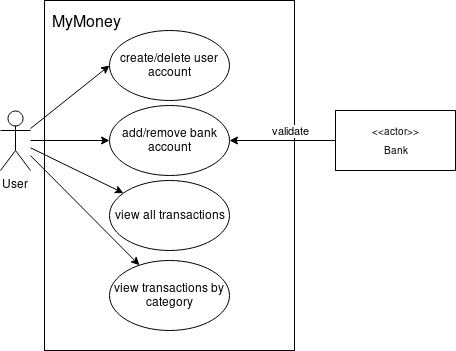
\includegraphics{UseCaseDiagram.png}
\caption{Use Case Diagram}
\label{fig:use-case-diagram}
\end{figure}

\begin{usecase}{Create User Account}
    \addrow{Case ID}{01}
    \addrow{Summary}{User gives information about a new user account, system validates it and creates the account.}
    \addrow{Scope}{money and budget management application}
    \addrow{Level}{user-goal}
    \addrow{Actors}{\textbf{User}}
    \addmulrow{Stakeholders and Interests}{
        \item User: Wants fast and easy account creation, clear and comprehensible display, proof of successful account creation.
        \item Company: Wants user interests to be fulfilled, wants to prevent erroneous input, wants fast communication with the local accountdatabase as well as fault tolerance in case of database conflicts, issues with editing authorisation, or other possible database problems.}
    \addrow{Pre-Conditions}{User has opened the application and is in the signup menu.}
    \addrow{Success Guarantee}{Account successfully saved in local account database, with name and password as specified by the user.}
    \addmulrow{Main Success Flow}{
        \item User enters a username, first name, last name, and password.
        \item System validates username and password (format, whether username is already used, etc).
        \item System creates new account.
        \item System notifies the user of the successful account creation, then returns to home menu.}
    \addrow{Exceptions}{}
    \addrow{Post-Conditions}{}
    \addrow{Priority}{}
    \addrow{Traces to Test Cases}{}
\end{usecase}

\begin{usecase}{Delete User Account}
    \addrow{Case ID}{02}
    \addrow{Summary}{User deletes a user account from the local accounts database, removing all bank accounts information associated with that account as well.}
    \addrow{Scope}{money and budget management application}
    \addrow{Level}{user-goal}
    \addrow{Actors}{\textbf{User}}
    \addmulrow{Stakeholders and Interests}{
        \item User: Wants easy navigation and secure account deletion, no risk of accidental deletion, proof of successful account deletion.
        \item Company: Wants user interests to be fulfilled, wants to ensure clean deletion from the database. }
    \addrow{Pre-Conditions}{User has logged in the user account he wants to delete.}
    \addrow{Success Guarantee}{user account is successfully deleted, all associated bank information is deleted, and user is returned to the home menu.}
    \addmulrow{Main Success Flow}{
        \item User enters the account settings, then selects 'delete account'.
        \item System brings up a confirmation menu to ensure that this selection was no accidentally entered.
        \item User affirms his choice.
        \item System successfully deletes all relevant entries in the local database, then notifies the user of this successful deletion.
        \item User confirms having read this notification.
        \item System brings the user back to the home menu.}
    \addrow{Exceptions}{}
    \addrow{Post-Conditions}{}
    \addrow{Priority}{}
    \addrow{Traces to Test Cases}{}
\end{usecase}


\begin{usecase}{Add Bank Account to a User Account}
    \addrow{Case ID}{03}
    \addrow{Summary}{User gives information about a new bank account, system sends it to the bank for verification then creates necessary entries in the local database once the bank approves the information.}
    \addrow{Scope}{money and budget management application}
    \addrow{Level}{user-goal}
    \addrow{Actors}{\textbf{User}, Bank}
    \addmulrow{Stakeholders and Interests}{
        \item User: Wants fast and easy account creation, clear and comprehensible display, proof of successful account creation.
        \item Company: Wants user interests to be fulfilled, wants to prevent erroneous input, wants fast communication with the local account database as well as the bank, wants fault tolerance in case of database conflicts, issues with the bank, or other possible local database problems.
        \item Bank: Wants to satisfy its customer base, wants correctly formatted account information given to its API, inexpensive and non-redundant communication of bank account data to third-party applications.}
    \addrow{Pre-Conditions}{User has logged in a user account and is in the user home menu.}
    \addrow{Success Guarantee}{Bank account successfully saved in local account database, with information corresponding the data validated by the bank.}
    \addmulrow{Main Success Flow}{
        \item User enters his/her bank account number.
        \item System validates input, and sends it to the bank for verification and connection`.
        \item Bank validates bank account number, and then responds with the bank account information.
        \item System records the valid bank account details securely in its database, and notifies the user of the successful addition of the bank account in the database.}
    \addrow{Exceptions}{}
    \addrow{Post-Conditions}{}
    \addrow{Priority}{}
    \addrow{Traces to Test Cases}{}
\end{usecase}

\begin{usecase}{Remove Bank Account from a User Account}
    \addrow{Case ID}{04}
    \addrow{Summary}{User deletes a bank account from the local database.}
    \addrow{Scope}{money and budget management application}
    \addrow{Level}{user-goal}
    \addrow{Actors}{\textbf{User}}
    \addmulrow{Stakeholders and Interests}{
        \item User: Wants easy navigation and secure account deletion, no risk of accidental deletion, proof of successful account deletion.
        \item Company: Wants user interests to be fulfilled, wants to ensure clean deletion from the database. }
    \addrow{Pre-Conditions}{User has logged in the user account whose active association with a bank account is the one the user wants to delete.}
    \addrow{Success Guarantee}{bank account is successfully removed from that user account, all associated bank information is deleted from the local database, and user is returned to the account home menu.}
    \addmulrow{Main Success Flow}{
        \item User selects the account he wants to remove, then selects 'remove account'.
        \item System brings up a confirmation menu to ensure that this selection was no accidentally entered.
        \item User affirms his choice.
        \item System successfully deletes all relevant entries in the local database, then notifies the user of this successful deletion.
        \item User confirms having read this notification.
        \item System brings the user back to the home account menu.}
    \addrow{Exceptions}{}
    \addrow{Post-Conditions}{}
    \addrow{Priority}{}
    \addrow{Traces to Test Cases}{}
\end{usecase}

\begin{usecase}{View Transactions for Specific Bank Account}
    \addrow{Case ID}{05}
    \addrow{Summary}{User selects specific bank account and views transactions associated with with selected bank account}
    \addrow{Scope}{money and budget management application}
    \addrow{Level}{user-goal}
    \addrow{Actors}{\textbf{User}}
    \addmulrow{Stakeholders and Interests}{
        \item User: Wants quick and convenient viewing of previous transactions from one specific bank account
  \item Company: Wants to give user ability to micromanage every aspect of the application down to each bank account and transaction.}
    \addrow{Pre-Conditions}{User has created and logged in a user account, and has added one or more bank accounts to his myMoney account. }
    \addrow{Success Guarantee}{User can view transaction by bank account.}
    \addmulrow{Main Success Flow}{
        \item User selects specific bank account from list of all accounts.
        \item System displays all previous transactions under specified bank account.
        \item User selects desired transaction.
        \item System shows all information about desired transaction, such as date and amount withdrawn, deposited, or transferred.}
    \addrow{Exceptions}{}
    \addrow{Post-Conditions}{}
    \addrow{Priority}{}
    \addrow{Traces to Test Cases}{}
\end{usecase}

\begin{usecase}{View All Transactions from all Bank Accounts}
    \addrow{Case ID}{06}
    \addrow{Summary}{User can view all transactions that have been made from all bank accounts}
    \addrow{Scope}{money and budget management application}
    \addrow{Level}{user-goal}
    \addrow{Actors}{\textbf{User}}
    \addmulrow{Stakeholders and Interests}{
        \item User: Wants easy and convenient viewing of all transactions among all bank accounts.
        \item Company: Wants user interests to be fulfilled.}
    \addrow{Pre-Conditions}{User has created and logged in a user account, and one or more bank accounts have been added to the system.}
    \addrow{Success Guarantee}{User is able to conveniently view all transactions from all institutions in one display.}
    \addmulrow{Main Success Flow}{
        \item User selects View All Transactions option.
        \item System shows all transactions across all accounts on one display.}
    \addrow{Exceptions}{}
    \addrow{Post-Conditions}{}
    \addrow{Priority}{}
    \addrow{Traces to Test Cases}{}
\end{usecase}

\begin{usecase}{View Transaction by Type}
    \addrow{Case ID}{07}
    \addrow{Summary}{User can view transactions by the following types: deposits, withdrawals, and transfers. }
    \addrow{Scope}{money and budget management application}
    \addrow{Level}{user-goal}
    \addrow{Actors}{\textbf{User}}
    \addmulrow{Stakeholders and Interests}{
        \item User: Wants to view transaction by type, such as withdrawals, deposits, and transfers for convenient view of the movement of his/her money throughout the accounts and accurate records of spending.
        \item Company: Wants user interests to be fulfilled. Wants to facilitate user?s ability to keep track of input and output of money between accounts.}
    \addrow{Pre-Conditions}{User has created and logged in a user account, added at least one bank account, and has made at least one type of transaction.}
    \addrow{Success Guarantee}{User is able to clearly view all deposits, withdrawals, and transfers that have been made.}
    \addmulrow{Main Success Flow}{
        \item User selects View All Transactions option or View By Specific Bank Account.
        \item System shows all transactions associated with previous choice.
        \item User selects view transactions by type
        \item System prompts user to choose which type of transaction he/she would like to view: deposits, withdrawals, transfers.
        \item User selects one of the options
        \item System shows all information regarding selected transaction such as date, amount, to which account, and from which account.}
    \addrow{Exceptions}{}
    \addrow{Post-Conditions}{}
    \addrow{Priority}{}
    \addrow{Traces to Test Cases}{}
\end{usecase}

\begin{usecase}{Categorize Transaction}
    \addrow{Case ID}{08}
    \addrow{Summary}{User can select a category to represent a transaction.}
    \addrow{Scope}{money and budget management application}
    \addrow{Level}{user-goal}
    \addrow{Actors}{\textbf{User}}
    \addmulrow{Stakeholders and Interests}{
        \item User: Wants to label each transaction as a specific type of spending, such as rent, bills, leisure, etc., to better manage and track spending habits.
        \item Company: Wants user interests to be fulfilled. Wants to facilitate user?s ability to budget and manage money through simple categorization of spending.}
    \addrow{Pre-Conditions}{User has created and logged in a user account, added at least one bank account, and has made at least one type of transaction.}
    \addrow{Success Guarantee}{User can quickly and efficiently categorize each transaction.}
    \addmulrow{Main Success Flow}{
        \item User selects desired transaction to categorize.
        \item User selects the + button.
        \item System displays the saved categories in a drop down menu.
        \item User selects preferred category to represent the current transaction.
        \item System saves transaction under chosen category.}
        \addrow{Exceptions}{}
    \addrow{Post-Conditions}{}
    \addrow{Priority}{}
    \addrow{Traces to Test Cases}{}
\end{usecase}

\begin{usecase}{View Transactions by Category}
    \addrow{Case ID}{09}
    \addrow{Summary}{User can view transaction according to categories of spending.}
    \addrow{Scope}{money and budget management application}
    \addrow{Level}{user-goal}
    \addrow{Actors}{\textbf{User}}
    \addmulrow{Stakeholders and Interests}{
        \item User: Wants to view transactions in different categories of spending such as rent, bills, leisure, etc., to view and monitor spending habits and allocate budget to each category of spending.
        \item Company: Wants to optimize the ease in which a user can allocate his/her budget, and track spending habits.}
    \addrow{Pre-Conditions}{User has created and logged in a user account, has added on or more bank accounts, has made at least one transaction and labeled the transaction according to which category it belongs.}
    \addrow{Success Guarantee}{User can easily categorize and view transactions.}
    \addmulrow{Main Success Flow}{
        \item User selects View All Transactions .
        \item System shows all transactions across all accounts on one display.
       \item User selects to view transaction by categories.
        \item System groups transactions by similar category.
        \item System displays transactions grouped by category.}
    \addrow{Exceptions}{}
    \addrow{Post-Conditions}{}
    \addrow{Priority}{}
    \addrow{Traces to Test Cases}{}
\end{usecase}


\section{Non-Functional Constraints}

\section{Data Dictionary}

\section{References}

\appendix

\section{Description of File Format: Tasks}

Describe input file format.

\section{Description of File Format: Persons}

Describe output file format.

\end{document}
